
%\chapter{Objectives}

\chapter{Context}

\section{Global change: how to describe the future of alpine ecosystems}

\subsection{The value of ecosystems}

\subsection{Global change}

\subsection{The need for mechanistic models}

\section{Community dynamics: complexity emerging from the parts and the role of phenotypic plasticity}

\subsection{The limit of classic patterns}

\subsection{The rise of individual-based approaches}

\subsection{When phenotypic plasticity makes things complicated}


%
%
%
%\section{Global change and community dynamics in alpine grasslands}
%\begin{figure*}
%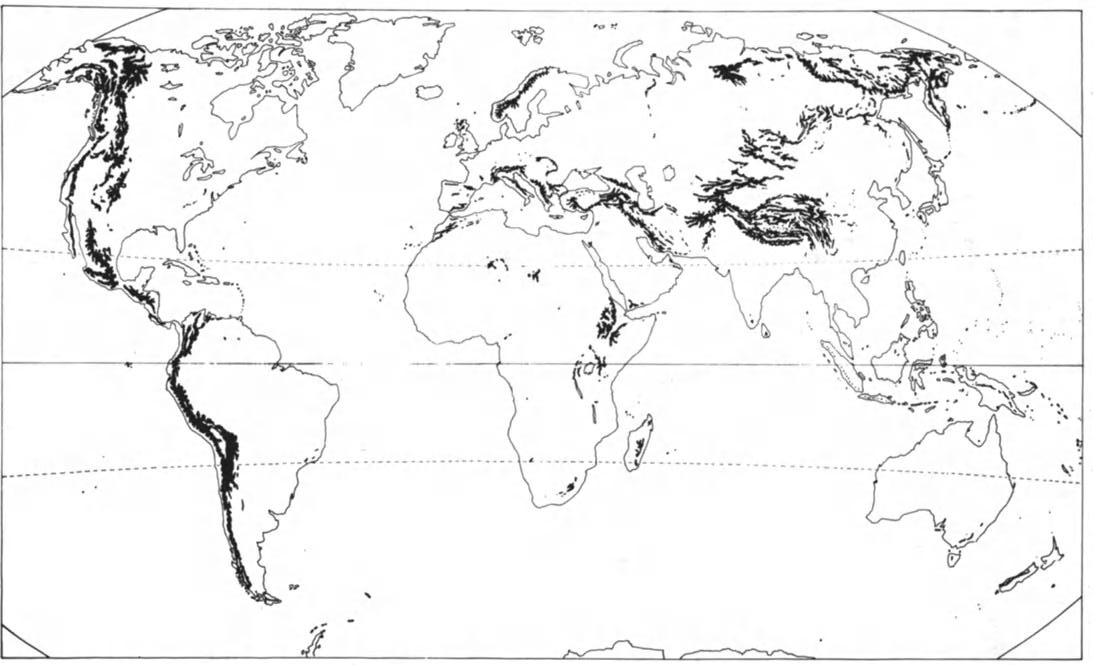
\includegraphics{./1_Introduction/graphics/alpine_distribution.jpeg}
%\caption{Distribution of alpine habitats}
%\end{figure*}
%
%Climate change is probably the greatest challenge the humanity has to face this century. Expected drastic changes in both average climatic conditions and punctual climatic event frequencies and intensities will, and already have, an impact all around the globe on multiple aspects of our lives. From agricultural and economic, to social and political, but also scientific and technical, the problems for human societies are numerous and multidimensional.\\ 
%Need to better understand and predict natural systems. Mountain grasslands are susceptible to be greatly impacted (even if certain think they might not). And in new ways as the rising temperature will certainly lead to migration to higher altitude, increasing the island characteristic of alpine habitats and reducing links between communities, and at the same time increasing the opportunity of invasion by lower altitude higher temperature species.\\
%\indent Detail a bit the characteristic of mountain grasslands, (snow, islands, grazing) the effect on species (snow-bed species, link to meta-community, diversity, species adaptation to frost etc... and how global change may affect that.\\
%\indent Because of that mountain grasslands are rich in species, but also vulnerable, that is why in parallel of predicting climate change, we also need to understand ecological mechanisms under this diversity and how they can be affected by global change \sidenote{section \ref{sec:coexistence}}. A key part in community diversity and in adaptation of communities also lies in the diversity and adaptation of individuals, so we are interested in intra-specific diversity and phenotypic plasticity \sidenote{section\ref{sec:intraspe}}.
%
%
%%Take home message ####################################
%\textbf{There is a need for new tools to predict the response of ecosystems to new climate conditions and management scenarios. These tools should integrate the complexity of such system and the mechanisms underlying the dynamic responses of these communities.}
%
%\section{Empirical results, trait approaches and need for a new kind of model in grasslands}
%
%\subsection{On trait-based approaches}
%
%Holy Graal of ecology\\
%Lavorel, Kraft, Kunstler
%
%\subsection{The importance of intra-specific variability}
%
%Jung
%Leps
%Albert
%Kichenin
%Lavorel (hypothesis of traits bell shape)
%Violle ...
%
%%Take home message ####################################
%\textbf{Trait approaches allow for generalisation and more direct link with processes and services. However they ignore variations and processes at lower levels than the species that are of critical importance for the understanding of community dynamics. A mechanistic approach integrating processes at the individual level and rich community complexity are needed.}
%
%\section{Close a gap in grassland modelling}
%
%%Take home message ####################################
%\textbf{Generalizing models for forest ecosystems and complex individual level models for grasslands coexist, but there is a need for a generalizing model at individual scale for grassland communities.}
%
%\section{Effect of phenotypic plasticity on coexistence and community dynamics}
%
%%Take home message ####################################
%\textbf{Despite empirical and theoretical work, the effects of intra-specific variability and plasticity on community dynamics are not fully disentangled. Understanding the effect of individual variations on plant community is crucial and may greatly alter how we envision the future of these ecosystems.}
%
%%_________________________________________________________________________________
%

\chapter{Aims, Objectives and Overview}
\section{Aims: functioning, diversity and flexibility}

Functioning
Diversity of : drivers, mechanisms, species and strategies
Flexibility: structure: genericity, experiments, plasticity

\section{Objectives: an agent-based model for plant community dynamics}

\subsection{Generic framework for multi-species and plastic plant modelling}
\subsection{Effect of phenotypic plasticity on plant growth and community dynamics}
\paragraph{Individual level}
\paragraph{Community level}

\section{Thesis overview}

Why the how: what makes these objectives valid\\
The machine\\
The results\\